\documentclass[c,aspectratio=169,14pt]{beamer}
\usetheme{C-SCALE}

\usepackage[sfdefault,lf]{carlito}
%\usepackage{pgf,pgfarrows,pgfnodes,pgfautomata,pgfheaps,pgfshade}
%\usepackage{amsmath,amssymb}
%\usepackage{xmpmulti}
\usepackage[utf8]{inputenc}
\usepackage[T1]{fontenc}
%\usepackage[czech]{babel}
\usepackage{tikz}
%\usepackage{colortbl,xspace}
\usepackage{tabularx}
\usepackage{mdframed}
%\usepackage{xcolor}
%\usepackage{eurosym}
\usepackage{ragged2e}
\usepackage{bbding}

\usepackage{ifthen}
\usepackage{contour}

\definecolor{activemqviolet}{cmyk}{.0,1.0,.50,.60}
\definecolor{awsorange}{RGB}{246,165,18}
\definecolor{azureblue}{RGB}{85,193,240}
\definecolor{ceritred}{RGB}{225,0,26}
\definecolor{cesnetblue}{RGB}{50,93,154}
\definecolor{dgorange}{RGB}{251,83,8}
\definecolor{eblue}{cmyk}{1,0.72,0,0.06}
\definecolor{egeeblue}{cmyk}{1,0.72,0,0.06}
\definecolor{egeeyellow}{cmyk}{0.0275,0.2588,0.9608,0.0039}
\definecolor{egiblack}{RGB}{0,0,0}
\definecolor{egiblue}{RGB}{0,103,177}
\definecolor{egigrey30}{RGB}{76,76,76}
\definecolor{egigrey50}{RGB}{128,128,128}
\definecolor{egigrey60}{RGB}{153,153,153}
\definecolor{egigrey70}{RGB}{179,179,179}
\definecolor{egiorange}{RGB}{200,113,0}
\definecolor{egrey}{cmyk}{0.02 0 0 0.05}
\definecolor{emiblue}{cmyk}{.98,.68,.35,.23}
\definecolor{emigrey}{cmyk}{0,0,0,.2}
\definecolor{emired}{cmyk}{.19,1,1,.12}
\definecolor{emiyellow}{cmyk}{.0,.25,1.00,.0}
\definecolor{egiblue}{RGB}{0,103,177}
\definecolor{eyellow}{cmyk}{0.0275,0.2588,0.9608,0.0039}
\definecolor{eyellowii}{cmyk}{0 0.02 0.08 0.1}
\definecolor{geantblue}{RGB}{0,68,91}
\definecolor{geantyellow}{RGB}{204,219,42}
\definecolor{globusblue}{RGB}{12,71,157}
\definecolor{globusorange}{RGB}{255,102,51}
\definecolor{hadoopblue}{RGB}{102,204,255}
\definecolor{indigoblue}{RGB}{7,44,98}
\definecolor{javablue}{RGB}{83,130,161}
\definecolor{javaorange}{RGB}{231,111,0}
\definecolor{lightyellow}{cmyk}{.0,.10,0.40,.0}
\definecolor{mavenorange}{RGB}{255,104,4}
\definecolor{metablue}{RGB}{67,138,196}
\definecolor{metagreendark}{RGB}{102,153,0}
\definecolor{metagreenlight}{RGB}{153,204,51}
\definecolor{metaorange}{RGB}{236,111,40}
\definecolor{metaviolet}{RGB}{102,102,153}
\definecolor{opennebulablue}{RGB}{0,145,197}
\definecolor{osgray}{RGB}{102,103,105}
\definecolor{osred}{RGB}{208,42,37}
\definecolor{owncloudblue}{RGB}{29,45,68}
\definecolor{rubyred}{RGB}{204,52,45}
\definecolor{snfgreen}{RGB}{0,165,81}
\definecolor{uvtbase}{RGB}{188,4,78}
\definecolor{slovakblue}{RGB}{11,78,162}
\definecolor{slovakred}{RGB}{238,28,37}
\definecolor{hueblue}{RGB}{40,125,189}
\definecolor{elixirorange}{RGB}{255,126,0}
\definecolor{michalyellow}{RGB}{255,255,0}
\definecolor{pear}{RGB}{209,226,49}
\definecolor{poopbrown}{RGB}{89,48,1}
\definecolor{pooppearyellow}{RGB}{184,176,17}
\definecolor{eoscblue}{RGB}{29,47,69}
\definecolor{eoscocre}{RGB}{180,134,45}
\definecolor{eudatblue}{RGB}{37,64,143}
\definecolor{deepyellow}{RGB}{246,183,38}
\definecolor{deepblue}{RGB}{68,79,156}


\newcommand{\aws}{\textcolor{awsorange}{AWS}}
\newcommand{\cerit}[1]{\textbf{\textsf{cer\leavevmode{\rlap{\textcolor{ceritred}{i}}\i}t#1}}}
\newcommand{\cesnet}[1]{\textbf{\textcolor{cesnetblue}{CESNET#1}}}
\newcommand{\datagrid}[1]{\textbf{\textcolor{dgorange}{Data}\textcolor{black}{Grid}#1}}
\newcommand{\egee}{\textcolor{egeeblue}{E}\textcolor{egeeyellow}{G}\textcolor{egeeblue}{EE}}
\newcommand{\egi}[1]{\textbf{\textcolor{egiblue}{EGI#1}}}
\newcommand{\emi}{\textsf{\textbf{\textcolor{emiblue}{EMI}}}}
\newcommand{\geant}{\textcolor{geantblue}{G\'{E}ANT}}
\newcommand{\glite}{\textcolor{egeeblue}{g}\textcolor{egeeyellow}{L}\textcolor{egeeblue}{ite}}
\newcommand{\hadoop}[1]{\textbf{\textit{\textcolor{hadoopblue}{\contour{black}{hadoop#1}}}}}
\newcommand{\indig}[1]{\ifthenelse{\equal{\unexpanded{#1}}{o}}{\textcolor{indigoblue}{\textbf{INDIGO}}}{\textcolor{indigoblue}{\textbf{Indig#1}}}}% requires: \usepackage{ifthen}
\newcommand{\jocci}{\textcolor{javaorange}{j}\textcolor{javablue}{OCCI}}
\newcommand{\LB}{L\&B\xspace}
\newcommand{\maven}{\textit{\textcolor{black}{\large m}\textcolor{mavenorange}{a}\textcolor{black}{ven}}}
\newcommand{\meta}[1]{\textbf{Meta\textcolor{metaorange}{#1}}}
\newcommand{\msazure}{\textcolor{azureblue}{MS Azure}}
\newcommand{\one}{{\large\textcolor{black}{o}\textcolor{opennebulablue}{ne}}}
\newcommand{\opennebul}[1]{\textcolor{black}{Open}\textcolor{opennebulablue}{Nebul#1}}
\newcommand{\openstack}[1]{\textsf{\textcolor{osgray}{open}\textcolor{osred}{stack}\textcolor{osgray}{#1}}}
\newcommand{\owncloud}[1]{\textsf{\textbf{\textcolor{owncloudblue}{ownCloud#1}}}}
\newcommand{\perun}[1]{\textbf{\textcolor{darkgray}{Perun#1}}}
\newcommand{\rocci}{\textcolor{rubyred}{r}\textcolor{opennebulablue}{OCCI}}
\newcommand{\synnef}[1]{\textit{\textcolor{snfgreen}{synnef#1}}}
\newcommand{\comfy}{\textcolor{rubyred}{COMFY}}
\newcommand{\itchy}{\textcolor{opennebulablue}{ITCHY}}
\newcommand{\nifty}{\textcolor{metaorange}{N\textcolor{darkgray}{I}FTY}}
%\newcommand{\michal}[1]{\textbf{\textcolor{michalyellow}{\contour{black}{MI}}\textcolor{pear}{\contour{black}{CH}}\textcolor{poopbrown}{\contour{black}{AL}}}#1}
\newcommand{\michal}[1]{\textbf{\textcolor{pooppearyellow}{MICHAL}#1}}
\newcommand{\hue}{\textbf{\textcolor{hueblue}{hue}}}
\newcommand{\elixir}[1]{\textit{\textcolor{black}{eli}\textcolor{elixirorange}{x}\textcolor{black}{ir#1}}}
\newcommand{\eoschub}[1]{\textcolor{eoscblue}{EOSC}\textcolor{eoscocre}{-hub#1}}
\newcommand{\whiteeoschub}[1]{\textcolor{white}{EOSC}\textcolor{eoscocre}{-hub#1}}
\newcommand{\eudat}[1]{\textcolor{eudatblue}{EUDAT#1}}
\newcommand{\deep}[1]{\textbf{\textcolor{deepyellow}{d}\textcolor{deepblue}{ee}\textcolor{deepyellow}{p#1}}}




%\usepackage{background}
%\backgroundsetup{
%    placement=center,
%    scale=5,
%    color=black,
%    contents={DRAFT},
%    opacity=.05
%}
%\setbeamertemplate{background}{\BgMaterial}%Uncomment for watermark



\begin{document}

\title{EO Metadata Query Service}
\subtitle{Efficient Discovery of Copernicus Data Assets}
\author{Stefan Reimond, EODC | Zdeněk Šustr, CESNET\\\textit{stefan.reimond@eodc.eu} | \textit{sustr4@cesnet.cz}}
\date{C-SCALE | 22~March 2023}

\begin{frame}[plain]
\vspace{8ex}
\maketitle
\end{frame}


\begin{frame}{Service Introduction}

EO-MQS (Earth Observation Metadata Query Service)
\begin{itemize}
\item Evolved from the original plan to federate Copernicus Data providers within C-SCALE
\begin{itemize}
\item \alert{Discovery} across the federation a major goal
\item \alert{Avoid} creating yet another matadata catalogue!
\item Data \alert{access} is outside the scope of the EO-MQS 
\end{itemize}
\item Main premise: partners already know where their data are
\begin{itemize}
\item Bring their discovery interfaces under a common one
\begin{itemize}
\item single point
\item shared protocol
\end{itemize}
\item describe their datasets and data retention policies
\item use that to pre-select candidates and redistribute user queries
\end{itemize}
\end{itemize}
\end{frame}



\begin{frame}{Datasets and Retention Policies}

\begin{itemize}
\item Acknowledge that different partners have different data
\begin{itemize}
\item National archives (full history, limited area)
\item Discipline archives (limited selection of product types, varying retention time)
\item Redistribution services (global coverage, short retention)
\item Big players (ambition to build global archive)
\end{itemize}
\item[$\implies$] Not every query needs to be redistributed to every partner
\begin{itemize}
\item Understand the query, select matching providers
\item Currently taking into account only product type
\begin{itemize}
\item \textit{Area} and \textit{time} filters not yet applied
\end{itemize}
\end{itemize}
\end{itemize}

\end{frame}



\begin{frame}{Providers' Catalogue}
\begin{itemize}
\item Called the \textit{EO Resource Catalogue} initially $\rightarrow$ confusion
\item Has \alert{only} provider information, not data (product) information
\begin{itemize}
\item Partners
\item Contacts
\item Services
\item Endpoints
\end{itemize}
\item Adopting the well known GOC-DB (\url{https://goc.egi.eu/})
\begin{itemize}
\item The ``Grid Configuration Database'', put to new uses
\item Keep track of members and relevant service endpoints\\{\scriptsize\url{https://goc.egi.eu/gocdbpi/public/?method=get_service_endpoint&scope=C-SCALE}}
\item Originally also intended for datasets and retention policies, but the choice of protocol changed that
\end{itemize}
\end{itemize}
\end{frame}

\begin{frame}{Choosing the Common Protocol}
\begin{itemize}
\item Choose from those already used in the federation?
\begin{itemize}
\item OpenSearch, OData, CWS, STAC
\item Then implement translation
\end{itemize}
\onslide<1>{
\item \alert{STAC} selected 
\begin{itemize}
\item modern protocol
\item lots of products supporting it
\item active community
\item \url{https://mqs.eodc.eu/stac/v1/}
\end{itemize}
\item Features
\begin{itemize}
\item Asset-focused: STAC breaks datasets into assets for easy data discovery.
\item Interoperability: STAC promotes compatibility with different tools and services.
\item Extensibility: STAC allows for custom metadata fields and extensions.
\end{itemize}}
\end{itemize}
\onslide<2>{
\begin{tikzpicture}[remember picture,overlay]
\node at (current page.center) {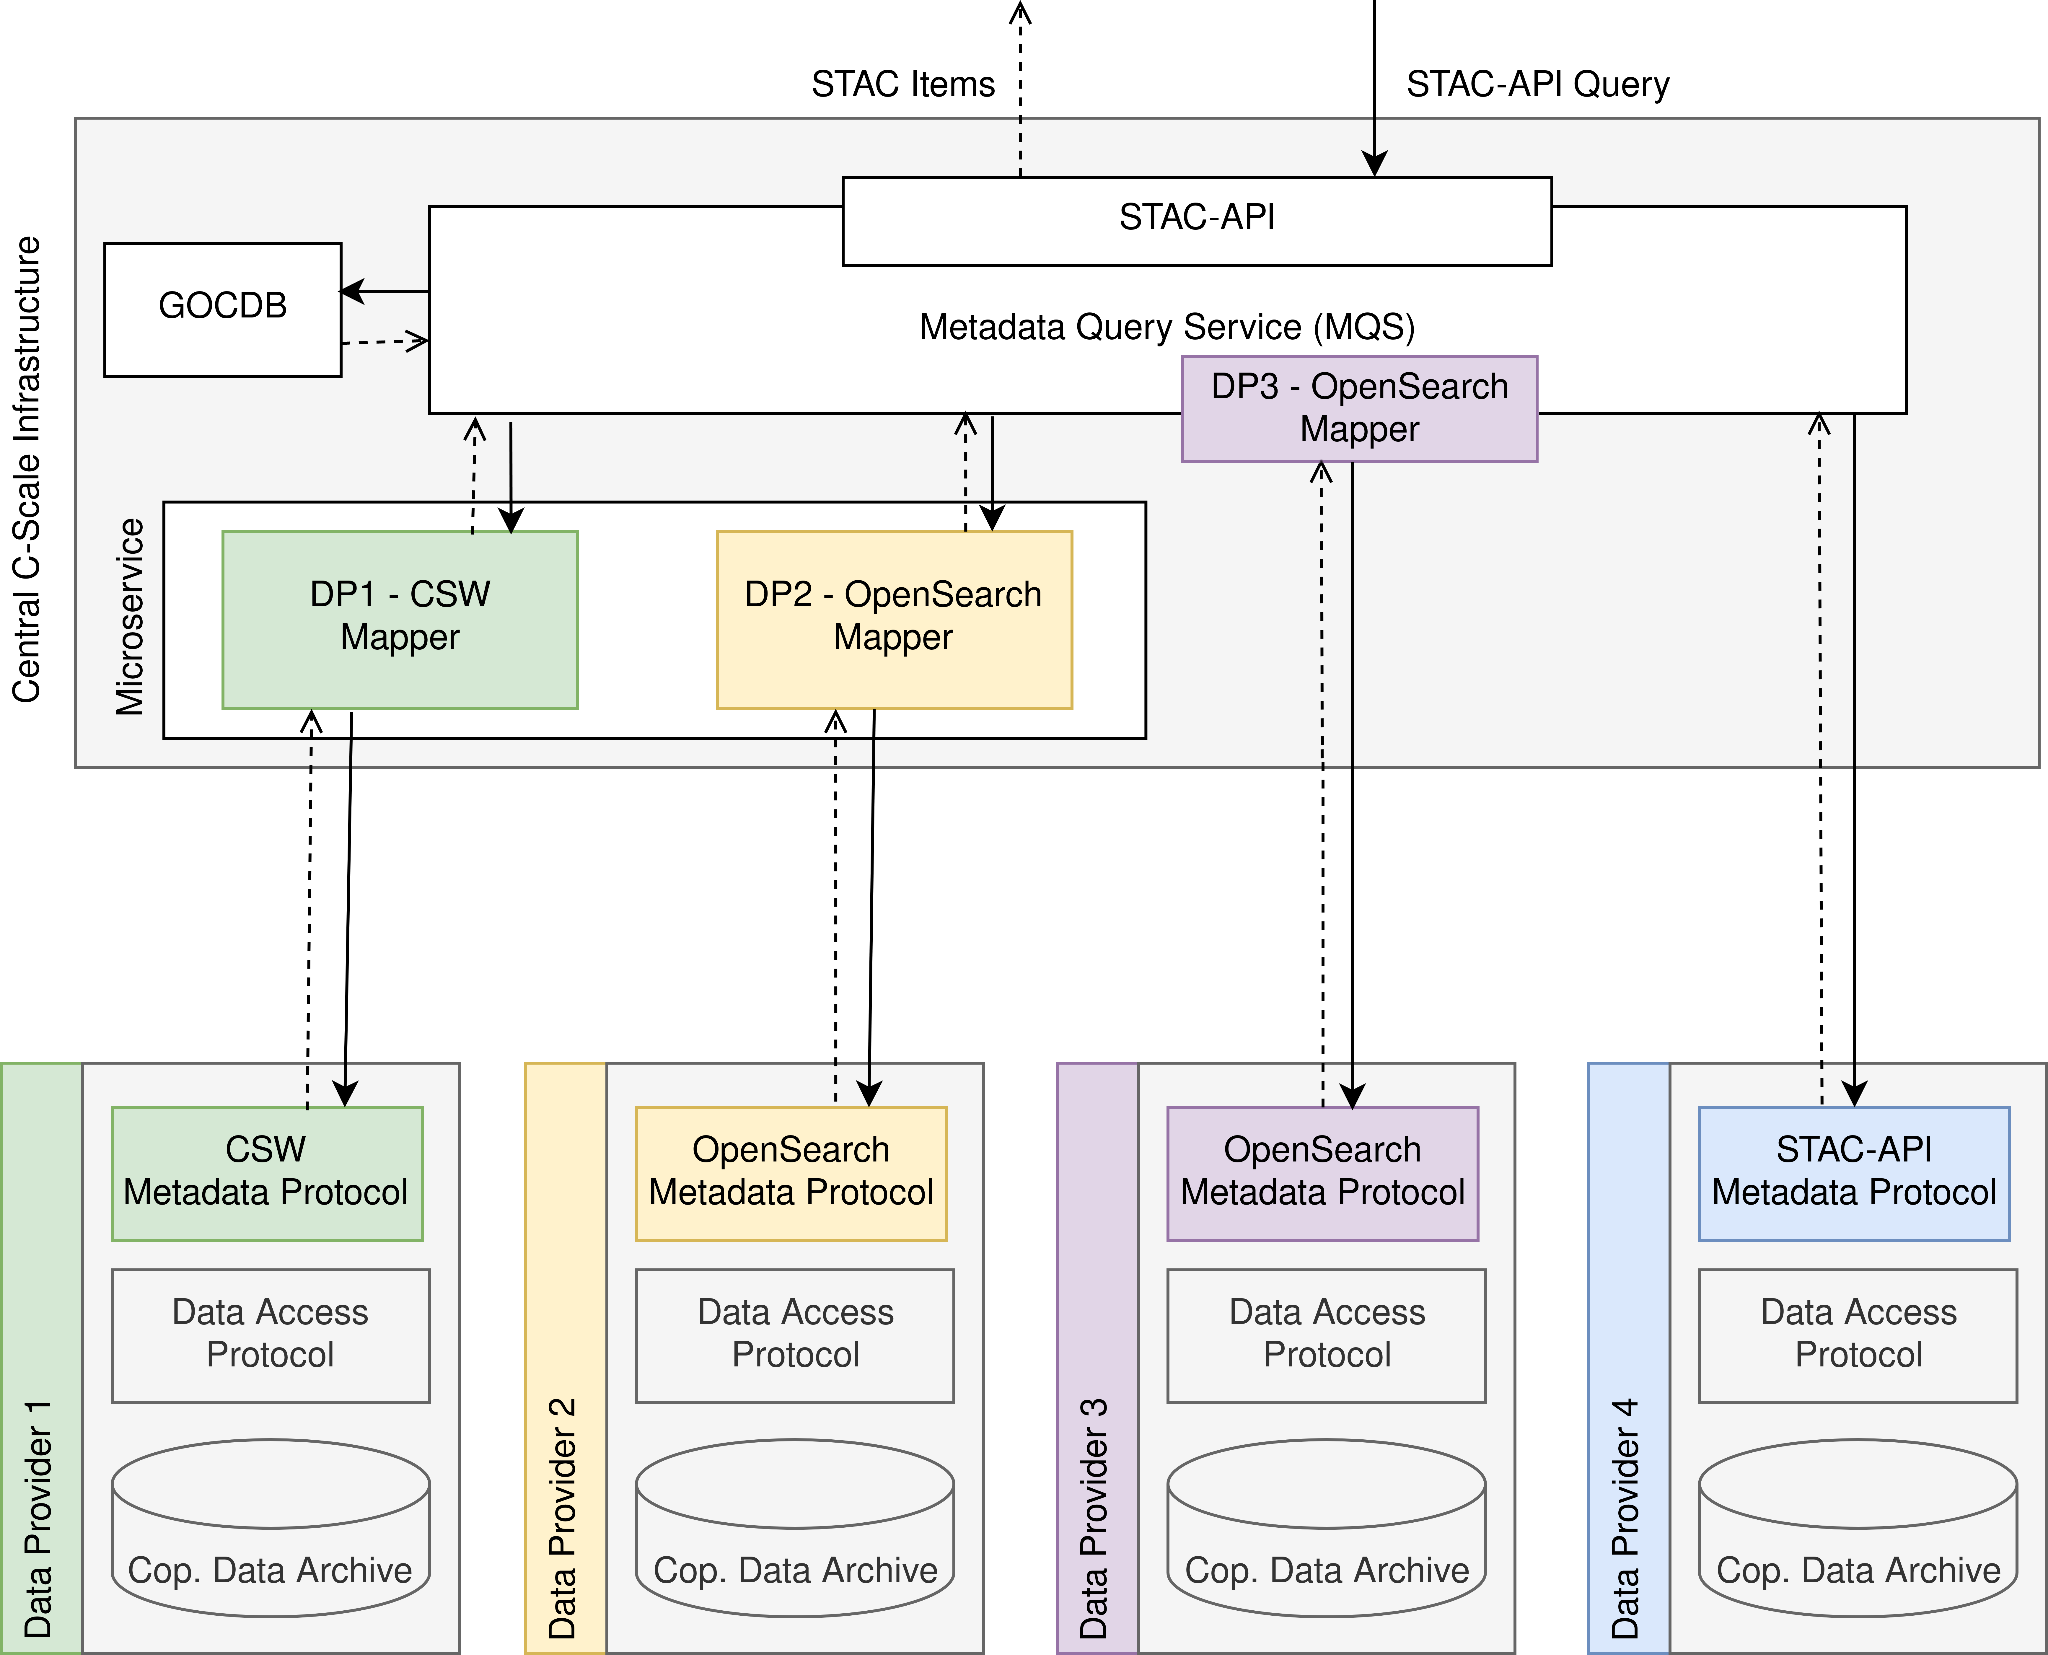
\includegraphics[height=.95\textheight]{img/d22-img001.png}};
\end{tikzpicture}}
\end{frame}


\begin{frame}{Demo: EO-MQS in Action}
\begin{itemize}
    \item Browsing and visualizing
    \begin{itemize}
    \item Get to know the EO-MQS in your browser with STAC Browser and other tools
    \end{itemize}  
    \item Working with the EO-MQS in Python
    \begin{itemize}
    \item Interact with EO-MQS programmatically in Jupyter notebooks.    
    \end{itemize}      
    \item Extra: how to become a data prvoider?
    \begin{itemize}
    \item Glance at the GOCDB
    \end{itemize}  
\end{itemize}      
Let's get started $\rightarrow$ \url{https://mqs.eodc.eu/help}  
\end{frame}




\begin{frame}{Challenges}
\begin{itemize}
\item Standardized STAC Collections structure?
\begin{itemize}
\item At least for members who are building new STAC databases, it might make sense to use a common collection structure
\end{itemize}
\item Paging
\begin{itemize}
\item How to handle item paging when multiple backends respond?
\item Cache and collate own pages? Send more than the query asked for?
\end{itemize}
\item Support of STAC API extensions?
\begin{itemize}
\item The EO-MQS officially supports the STAC API Core parmaters
\item API Extension with filtering functionality is valuable, but hard to realize across federation
\end{itemize}
\end{itemize}
\end{frame}


\begin{frame}{Outlook}
    \begin{itemize}
    \item Constant improvement of EO-MQS package
    \begin{itemize}
        \item New features
        \item Fixing bugs 
        \item Better documentation
    \end{itemize}
    \item Release of STAC Browser v3
    \begin{itemize}
    \item Recently published, allows searching and filtering in the browser
    \item Will be deployed soon at \url{https://mqs.eodc.eu/browser} 
    \end{itemize}
    \item EOSC Service Onboarding
    \begin{itemize}
    \item The EO-MQS is presently undergoing onboarding as an EOSC service
    \end{itemize}
    \end{itemize}
    \end{frame}
\begin{finalframe}
\hfill Thank you\hfill\null

\medskip
\hfill \large Questions?\hfill\null

\end{finalframe}

\end{document}
